% generated by Docutils <http://docutils.sourceforge.net/>
\documentclass[english]{article}
\usepackage{fixltx2e} % LaTeX patches, \textsubscript
\usepackage{cmap} % fix search and cut-and-paste in PDF
\usepackage[T1]{fontenc}
\usepackage[utf8]{inputenc}
\usepackage{ifthen}
\usepackage{babel}
\usepackage[margin=1.0in]{geometry}
\usepackage{longtable}
\usepackage{array}
\setlength{\extrarowheight}{2pt}
\newlength{\DUtablewidth} % internal use in tables

% transition (break, fancybreak, anonymous section)
\providecommand*{\DUtransition}[1][class-arg]{%
  \hspace*{\fill}\hrulefill\hspace*{\fill}
  \vskip 0.5\baselineskip
}


%%% Custom LaTeX preamble

%\parindent=0pt
%\parsep=10pt
\setlength{\parindent}{0pt}
\setlength{\parskip}{6pt plus 2pt minus 1pt}

% PDF Standard Fonts
\usepackage{mathptmx} % Times
\usepackage[scaled=.90]{helvet}
\usepackage{courier}
%%% User specified packages and stylesheets
\usepackage{graphicx}

\renewcommand{\familydefault}{cmss}
\renewcommand{\bf}{\bfseries}

%%% Fallback definitions for Docutils-specific commands
% fieldlist environment
\ifthenelse{\isundefined{\DUfieldlist}}{
  \newenvironment{DUfieldlist}%
    {\quote\description}
    {\enddescription\endquote}
}{}

% hyperlinks:
\ifthenelse{\isundefined{\hypersetup}}{
  \usepackage[unicode,colorlinks=true,linkcolor=blue,urlcolor=blue,bookmarks]{hyperref}
  \urlstyle{same} % normal text font (alternatives: tt, rm, sf)
}{}


% inline markup (custom roles)
% \DUrole{#1}{#2} tries \DUrole#1{#2}
\providecommand*{\DUrole}[2]{%
  \ifcsname DUrole#1\endcsname%
    \csname DUrole#1\endcsname{#2}%
  \else% backwards compatibility: try \docutilsrole#1{#2}
    \ifcsname docutilsrole#1\endcsname%
      \csname docutilsrole#1\endcsname{#2}%
    \else%
      #2%
    \fi%
  \fi%
}

%%% Body
\begin{document}

\begin{titlepage}
\title{{\Huge Seismic Analysis Code\\
Users Manual}}
\date{\today}
\author{Version 101.6a}
\maketitle

\begin{center} \

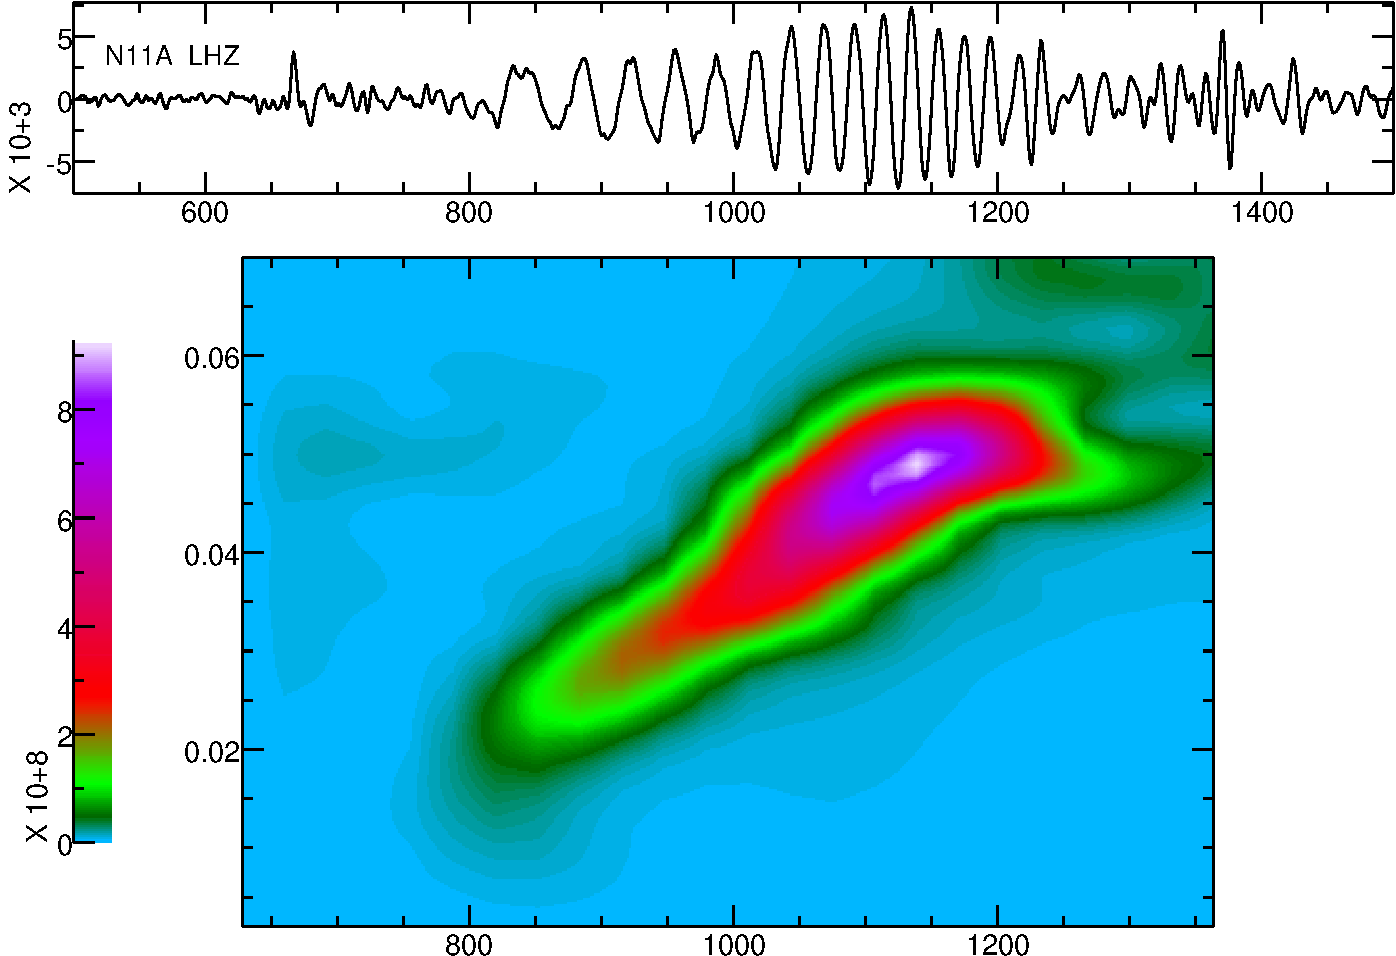
\includegraphics[width=0.9\linewidth]{./sac_spectrogram.pdf}
\end{center}

{\Large Sections}

\begin{itemize}
\item Using SAC
\item SAC Commands
\item Signal-Stacking Subprocess
\item Spectral-Estimation Subprocess
\end{itemize}

\end{titlepage}

\tableofcontents

\newpage
\section{Using SAC
\label{using_sac}
}
\input{manual/intro}
\include{manual/tutorial}
\include{manual/analysis}
\include{manual/sac_macros}
\include{manual/inline}
\include{manual/file_format}
\include{manual/input_output}
\include{manual/saclib}
\include{manual/blackboard}
\include{manual/graphics}
\include{manual/sgf_format}
\include{manual/sac_script}
\include{manual/error_messages}
\newpage
\section{SAC Commands
\label{sac_commands}
}
\input{commands/alpha_commands}
\include{commands/3c}
\include{commands/about}
\include{commands/absolutevalue}
\include{commands/add}
\include{commands/addf}
\include{commands/apk}
\include{commands/arraymap}
\include{commands/axes}
\include{commands/bandpass}
\include{commands/bandrej}
\include{commands/bbfk}
\include{commands/beam}
\include{commands/begindevices}
\include{commands/beginframe}
\include{commands/beginwindow}
\include{commands/benioff}
\include{commands/binoperr}
\include{commands/border}
\include{commands/capf}
\include{commands/chnhdr}
\include{commands/chpf}
\include{commands/color}
\include{commands/comcor}
\include{commands/contour}
\include{commands/convert}
\include{commands/convolve}
\include{commands/copyhdr}
\include{commands/correlate}
\include{commands/crr}
\include{commands/cut}
\include{commands/cuterr}
\include{commands/cutim}
\include{commands/datagen}
\include{commands/decimate}
\include{commands/deletechannel}
% \include{commands/depmec}
\include{commands/dif}
\include{commands/div}
\include{commands/divf}
\include{commands/divomega}
\include{commands/echo}
\include{commands/enddevices}
\include{commands/endframe}
\include{commands/envelope}
\include{commands/erase}
\include{commands/evaluate}
\include{commands/exp}
\include{commands/exp10}
\include{commands/external_howto}
\include{commands/external_interface}
\include{commands/fft}
\include{commands/fileid}
\include{commands/filenumber}
\include{commands/filterdesign}
\include{commands/fir}
\include{commands/floor}
\include{commands/funcgen}
\include{commands/getbb}
\include{commands/grayscale}
\include{commands/grid}
\include{commands/gtext}
\include{commands/hanning}
\include{commands/help}
\include{commands/highpass}
\include{commands/hilbert}
\include{commands/history}
\include{commands/hlpintro}
\include{commands/ifft}
\include{commands/image}
\include{commands/inicm}
\include{commands/installmacro}
\include{commands/int}
\include{commands/interpolate}
\include{commands/intro}
\include{commands/keepam}
\include{commands/khronhite}
\include{commands/line}
\include{commands/linefit}
\include{commands/linlin}
\include{commands/linlog}
\include{commands/listhdr}
\include{commands/load}
\include{commands/loadctable}
\include{commands/log}
\include{commands/log10}
\include{commands/loglab}
\include{commands/loglin}
\include{commands/loglog}
\include{commands/lowpass}
\include{commands/macro}
\include{commands/map}
\include{commands/markptp}
\include{commands/marktimes}
\include{commands/markvalue}
\include{commands/mat}
\include{commands/mathop}
\include{commands/merge}
\include{commands/message}
\include{commands/mtw}
\include{commands/mul}
\include{commands/mulf}
\include{commands/mulomega}
\include{commands/nplotc}
\include{commands/null}
\include{commands/oapf}
\include{commands/ohpf}
\include{commands/pause}
\include{commands/pickauthor}
\include{commands/pickphase}
\include{commands/pickprefs}
\include{commands/picks}
\include{commands/plabel}
\include{commands/plot}
\include{commands/plot1}
\include{commands/plot2}
\include{commands/plotalpha}
\include{commands/plotc}
\include{commands/plotctable}
\include{commands/plotdy}
\include{commands/plotpk}
\include{commands/plotpktable}
\include{commands/plotpm}
\include{commands/plotsp}
\include{commands/plotxy}
\include{commands/print}
\include{commands/printhelp}
\include{commands/production}
\include{commands/qdp}
\include{commands/quantize}
\include{commands/quit}
\include{commands/quitsub}
\include{commands/read}
\include{commands/readbbf}
\include{commands/readcss}
\include{commands/readdb}
\include{commands/readerr}
\include{commands/readgse}
\include{commands/readhdr}
\include{commands/readsdd}
\include{commands/readsp}
\include{commands/readsuds}
\include{commands/readtable}
\include{commands/report}
\include{commands/reverse}
\include{commands/rglitches}
\include{commands/rmean}
\include{commands/rms}
\include{commands/rotate}
\include{commands/rq}
\include{commands/rtrend}
\include{commands/saveimg}
\include{commands/scallop}
\include{commands/setbb}
\include{commands/setdevice}
\include{commands/setmacro}
\include{commands/sgf}
\include{commands/smooth}
\include{commands/sonogram}
\include{commands/sort}
\include{commands/spectrogram}
\include{commands/sqr}
\include{commands/sqrt}
\include{commands/stretch}
\include{commands/sub}
\include{commands/subf}
\include{commands/symbol}
\include{commands/synchronize}
\include{commands/systemcommand}
\include{commands/taper}
\include{commands/ticks}
\include{commands/title}
\include{commands/trace}
\include{commands/transcript}
\include{commands/transfer}
\include{commands/transfertable}
\include{commands/traveltime}
\include{commands/tsize}
\include{commands/unsetbb}
\include{commands/unwrap}
\include{commands/vspace}
\include{commands/wait}
\include{commands/whiten}
\include{commands/whpf}
\include{commands/width}
\include{commands/wiener}
\include{commands/wild}
\include{commands/window}
\include{commands/write}
\include{commands/writebbf}
\include{commands/writecss}
\include{commands/writegse}
\include{commands/writehdr}
\include{commands/writesdd}
\include{commands/writesp}
\include{commands/xdiv}
\include{commands/xfudge}
\include{commands/xfull}
\include{commands/xgrid}
\include{commands/xlabel}
\include{commands/xlim}
\include{commands/xlin}
\include{commands/xlog}
\include{commands/xvport}
\include{commands/ydiv}
\include{commands/yfudge}
\include{commands/yfull}
\include{commands/ygrid}
\include{commands/ylabel}
\include{commands/ylim}
\include{commands/ylin}
\include{commands/ylog}
\include{commands/yvport}
\include{commands/zcolors}
\include{commands/zlabels}
\include{commands/zlevels}
\include{commands/zlines}
\include{commands/zticks}

\newpage
\section{Signal-Stacking Subprocess
\label{`signal-stacking subprocess manual`}
}
\input{commands/sss.com/sss}
\include{commands/sss.com/addstack}
\include{commands/sss.com/changestack}
\include{commands/sss.com/deletestack}
\include{commands/sss.com/deltacheck}
\include{commands/sss.com/distanceaxis}
\include{commands/sss.com/distancewindow}
\include{commands/sss.com/globalstack}
\include{commands/sss.com/incrementstack}
\include{commands/sss.com/liststack}
\include{commands/sss.com/plotrecordsection}
\include{commands/sss.com/plotstack}
\include{commands/sss.com/sumstack}
\include{commands/sss.com/timeaxis}
\include{commands/sss.com/timewindow}
\include{commands/sss.com/traveltime}
\include{commands/sss.com/velocitymodel}
\include{commands/sss.com/velocityroset}
\include{commands/sss.com/writestack}
\include{commands/sss.com/zerostack}

\newpage
\section{Spectral-Estimation Subprocess
\label{`spectral-estimation subprocess manual`}
}
\input{commands/spe.com/spe}
\include{commands/spe.com/cor}
\include{commands/spe.com/mem}
\include{commands/spe.com/mlm}
\include{commands/spe.com/pds}
\include{commands/spe.com/plotcor}
\include{commands/spe.com/plotpe}
\include{commands/spe.com/plotspe}
\include{commands/spe.com/quitsub}
\include{commands/spe.com/read}
\include{commands/spe.com/readcor}
\include{commands/spe.com/writecor}
\include{commands/spe.com/writespe}

\end{document}
